\documentclass[conference]{IEEEtran}
\IEEEoverridecommandlockouts
% The preceding line is only needed to identify funding in the first footnote. If that is unneeded, please comment it out.
\usepackage{cite}
\usepackage{amsmath,amssymb,amsfonts}
\usepackage{algorithmic}
\usepackage{graphicx}
\usepackage{textcomp}
\usepackage{xcolor}
\usepackage{booktabs}
\usepackage{tabularx}
\def\BibTeX{{\rm B\kern-.05em{\sc i\kern-.025em b}\kern-.08em
    T\kern-.1667em\lower.7ex\hbox{E}\kern-.125emX}}
\begin{document}

\title{A Comparative Evaluation of Encoder and Decoder Language Models with Parameter-Efficient Fine-Tuning (PEFT/LoRA) 
for Multi-Class Text Emotion Recognition
}

\author{\IEEEauthorblockN{Francisco Kuo Liu}
\IEEEauthorblockA{\textit{School of Computer Engineering} \\
\textit{Instituto Tecnológico de Costa Rica}\\
Cartago, Costa Rica \\
fkuo@estudiantec.cr}
\and
\IEEEauthorblockN{Jimmy Feng Liu}
\IEEEauthorblockA{\textit{School of Computer Engineering} \\
\textit{Instituto Tecnológico de Costa Rica}\\
Cartago, Costa Rica \\
jfeng@estudiantec.cr}
\and
\IEEEauthorblockN{Danielo Wu Zhong}
\IEEEauthorblockA{\textit{School of Computer Engineering} \\
\textit{Instituto Tecnológico de Costa Rica}\\
Cartago, Costa Rica \\
dwu@estudiantec.cr}
}

\maketitle

\begin{abstract}
We present a controlled benchmark of eight models for six-class emotion recognition on a leakage-controlled version of a CARER-derived corpus. All models train on the same 32,000-text subset and are scored once on the same 37,153 test texts: a TF-IDF baseline, a BiLSTM with GloVe, two fully fine-tuned encoders (DistilBERT, BERT-base), and four decoders adapted with QLoRA (Qwen2.5-0.5B, Qwen2.5-1.5B, Gemma 4 E2B, DeepSeek-R1-Distill-Qwen-1.5B). BERT-base is the best model (Macro-F1 $0.9895 \pm 0.0005$ over three seeds), and the top five models lie within $0.0021$ of each other. A paired bootstrap finds a systematic $0.034$ gap between Qwen2.5-1.5B and Gemma 4 E2B, and no consistent difference between the two encoders, between the two Qwen2.5 sizes, or between Qwen2.5-1.5B and its reasoning-distilled counterpart. The five best models make 59\% to 61\% of their errors on the 1.5\% of test texts that lack the dominant ``feel'' phrasing. Integrated Gradients on BERT-base show that removing the single most attributed word changes the prediction in 75\% of the texts (7\% for a random word), and that this word is a class-marker term in 77.5\% of them, in line with the lexical cues that a linear model also exploits.
\end{abstract}

\begin{IEEEkeywords}
Text Emotion Recognition, Large Language Models, LoRA, PEFT, Macro-F1, Multi-class Classification.
\end{IEEEkeywords}

\section{Introduction}
Text-based emotion recognition is central to applications ranging from conversational agents to consumer feedback analysis and mental health monitoring. 
However, reliably detecting fine-grained emotional states in brief, informal digital texts remains difficult due to contextual ambiguity and severe 
class imbalance. While recurrent models like BiLSTM and encoder-based architectures like BERT have long served as primary baselines, generative 
Large Language Models (LLMs) have demonstrated strong potential in capturing complex semantic variations through advanced pre-training. Despite this 
potential, the massive parameter size of modern decoders makes full fine-tuning computationally unfeasible for resource-constrained environments, 
highlighting the need for efficient adaptation techniques.

Parameter-Efficient Fine-Tuning (PEFT) methods, particularly Low-Rank Adaptation (LoRA), address these hardware bottlenecks by freezing the 
pre-trained base model and updating only a small subset of low-rank adapter weights. Although decoders such as Qwen, Gemma, and DeepSeek excel 
in general language tasks, their performance when adapted via LoRA for specialized downstream classification under high class imbalance is not 
yet fully understood. Existing benchmarks often focus on broad sentiment analysis or general classification, relying on overall accuracy, a metric 
that frequently masks poor performance on minority emotional classes. Furthermore, direct comparisons between fully fine-tuned lightweight encoders 
and LoRA-adapted intermediate decoders under identical hardware constraints remain scarce in current literature.

To address these gaps, this work evaluates the trade-offs between legacy encoder baselines and modern intermediate-scale decoders on the highly 
imbalanced CARER emotion dataset.

Building on this motivation, our guiding research question is the following: how do architectural family, parameter scale, and training objective each affect the trade-off between classification quality (Macro-F1) and computational cost in multi-class emotion classification, and which of these three factors most strongly influences that trade-off? Rather than searching for a single winning architecture, this work isolates each factor through matched comparisons, allowing its individual contribution to be characterized independently of the others.

\textbf{Working Hypothesis:} We hypothesize that \textit{parameter scale} and \textit{training objective} yield diminishing returns for 
fine-grained multi-class emotion classification, whereas the \textit{architectural family} (generative decoder vs. discriminative encoder) 
dominates performance. Specifically, we predict that a 1.5B LoRA-adapted generative decoder (Qwen2.5-1.5B) will achieve higher Macro-F1 scores 
on minority emotion classes (e.g., \textit{surprise}, \textit{love}) than fully fine-tuned encoders (BERT-Base), but that increasing decoder scale 
beyond 2B parameters will yield marginal Macro-F1 gains while disproportionately increasing peak VRAM footprint and inference latency. The executed study drops Gemma 4 E4B (Section~\ref{sec:method2}), so that larger-scale comparison is not in the reported runs, and inference latency was not measured.

Our main contributions are as follows:
\begin{itemize}
    \item \textbf{Three-Axis Controlled Benchmark:} We design a controlled comparison that isolates architectural family, parameter scale, and training objective as independent variables, rather than benchmarking architectures in an unstructured manner.
    \item \textbf{Efficiency \& Optimization Analysis:} We evaluate the operational trade-offs of PEFT/LoRA across decoder architectures, focusing on memory footprint, parameter count, and convergence rates under strict hardware limitations.
    \item \textbf{Imbalance-Aware Evaluation:} We analyze model resilience to severe class imbalance on the CARER dataset, prioritizing Macro-F1 metrics to ensure fair assessment across underrepresented emotion classes.
    \item \textbf{Practical Deployment Guidelines:} We outline concrete performance-versus-compute trade-offs to offer actionable decision frameworks for researchers and practitioners choosing between compact encoders and LoRA-adapted decoders.
\end{itemize}

The remainder of this paper is structured as follows: Section~\ref{sec:ejeA} reviews the evolution and current approaches in text-based emotion recognition. Section~\ref{sec:ejeB} analyzes parameter-efficient adaptation methods across Encoder and Decoder architectures. Section~\ref{sec:ejeC} examines the benchmark dataset characteristics and evaluation protocols. Section~\ref{sec:method2} describes the experimental methodology that was executed. Section~\ref{sec:results2} reports the results, Section~\ref{sec:limits2} states the limitations, Section~\ref{sec:discussion} discusses the trade-offs, and Section~\ref{sec:conclusion} concludes the paper.

\section{Domain Analysis \& Evolution of Text Emotion Recognition}
\label{sec:ejeA}
\subsection{Dominant Traditional Approaches}
Text-based emotion recognition (TBED) has evolved through a rapid progression of computational methodologies designed to address semantic ambiguity and unstructured language. Affective computing has transitioned from rule-based and lexicon-driven heuristics toward deep representation learning and generative paradigms \cite{maruf2024challenges}. 
Some of these computational approaches have relied on multiple computational paradigms to interpret a text and determine which emotions are shown. 
These foundational techniques can be broadly categorized into keyword-based, corpus-based, rule-based, traditional machine learning, and deep learning:

\begin{itemize}
    \item \textbf{Keyword-Based Approaches}: Identify explicit emotional terms using lexical databases (such as WordNet-Affect or SentiWordNet) and apply linguistic rules to assess sentiment intensity \cite{murthy2021review}.
    
    \item \textbf{Corpus-Based Approaches}: Induce domain-specific word-emotion lexicons using statistical methods and generative models across annotated or weakly-labeled text datasets \cite{murthy2021review}.
    
    \item \textbf{Rule-Based Approaches}: Apply expert heuristic rules, Part-of-Speech tagging, and phrasal patterns to infer emotional states based on predefined linguistic structure \cite{murthy2021review}.
    
    \item \textbf{Traditional Machine Learning Approaches}: Utilize supervised algorithms, such as, Support Vector Machines (SVM), Na\"ive Bayes, Decision Trees, and $K$-Nearest Neighbors that rely on manual feature engineering to classify text into emotional categories \cite{murthy2021review}.
    
    \item \textbf{Deep Learning Approaches}: Employ neural network architectures, such as, Recurrent Neural Networks (RNNs/LSTMs), Convolutional Neural Networks (CNNs), and Transformer-based models (e.g., BERT), to automatically learn hierarchical representations and capture complex contextual semantics directly from raw text [1].
\end{itemize}

\subsection{The Shift to Generative Decoders}

The rise of generative Large Language Models (LLMs) has fundamentally changed how we approach text classification in NLP \cite{chakriswaran2019emotion}. 
Traditionally, affective computing tasks relied on discriminative models that learn a direct mapping function $f(X) \to Y$ 
from input text $X$ to a predefined set of labels $Y$ \cite{saravia2018carer}. In contrast, autoregressive decoder architectures treat classification 
as a conditional text generation problem. They model the probability of generating a target class token $y$ given a prompt sequence $X$:

\begin{equation}
    P(y \mid X) = \prod_{i=1}^{N} P(w_i \mid w_{1}, \dots, w_{i-1}, X)
\end{equation}

\noindent This shift offers significant benefits, especially when it comes to leveraging broad contextual knowledge and picking up on subtle 
emotional tone in short informal text \cite{kratzwald2018deep}.

\subsubsection{Zero-Shot and Few-Shot Prompting Paradigms}
A key feature of generative decoders is their ability to handle downstream classification without updating model weights, 
relying instead on in-context learning (ICL) \cite{cheng2026personality}. In a zero-shot setup, the model gets an instruction 
template describing the task along with the input text, using its pre-trained knowledge to output the predicted label. 
Few-shot prompting builds on this by adding $k$ example pairs directly into the prompt context:

\begin{equation}
    \text{Prompt} = \{ (X_1, Y_1), (X_2, Y_2), \dots, (X_k, Y_k), X_{\text{test}} \}
\end{equation}

While zero-shot and few-shot setups avoid task-specific training costs, their reliability for fine-grained emotion tasks varies greatly. 
Zero-shot decoders are notoriously sensitive to how prompts are written, how context examples are ordered, and how subtle affective 
context is presented. Furthermore, without parameter adaptation for a specific domain, zero-shot LLMs often struggle with subtle emotion boundaries.
Furthermore, empirical studies comparing small task-specific encoders against 7B generative models (e.g., Llama-2 and Mistral) show that in-context prompting often yields higher variance and lower overall classification accuracy on affective tasks compared to direct supervised tuning \cite{stigall2024large}.

\subsubsection{Supervised Fine-Tuning versus In-Context Learning}
To address the instability of in-context learning, supervised fine-tuning (SFT) adjusts the model's output probabilities to align 
directly with task-specific labels. In multi-class emotion recognition, SFT restricts the output space to valid emotion categories 
while teaching the model to handle informal digital slang and implicit emotional cues \cite{kratzwald2018deep}.

However, choosing between prompting and full fine-tuning presents clear trade-offs:

\begin{itemize}
    \item \textbf{In-Context Learning (Zero/Few-Shot):} Keeps base weights frozen and avoids training costs, but can struggle with subtle emotional nuances.
    \item \textbf{Full Supervised Fine-Tuning (SFT):} Delivers strong task alignment across imbalanced emotion classes, but requires updating billions of parameters ($>10^9$), creating massive computational and memory bottlenecks during backpropagation.
\end{itemize}

This balance demonstrates why intermediate approaches are necessary. Generative decoders provide strong semantic understanding, 
but using them effectively for emotion classification requires parameter-efficient strategies, such as Low-Rank Adaptation (LoRA), 
that deliver SFT performance without excessive computational demands \cite{nwaiwu2025peft}.

\subsection{Established Standards and Open Challenges}
Sentiment analysis and emotion recognition overlap significantly in computational linguistics, but they present very different levels of 
complexity. Distinguishing basic sentiment classification from fine-grained emotion recognition makes it easier to pinpoint the key 
challenges facing modern NLP.

\subsubsection{Published Recurrent Results}
Binary sentiment classification, which sorts text into positive or negative categories, is a different task from six-class emotion recognition.
Zhang \cite{zhang2024comparative} compares RNN, GRU, and LSTM variants, including bidirectional models, on a Kaggle Twitter set of six emotions after downsampling every class to the same size (20\% of the data held out for testing). BERT and DistilBERT are named in the introduction of that paper; the trained models are recurrent. On the balanced sample, Table 1 reports a two-layer Bi-LSTM at test accuracy 0.9321 and F1 0.93 after 200 epochs, and a two-layer Bi-GRU at accuracy 0.8833 and F1 0.88. Those accuracies describe the balanced sample.

\subsubsection{Open Challenge 1: Fine-Grained Multi-Class Emotion Mapping}
Moving beyond binary sentiment requires mapping text to specific psychological states. This work uses six categories: joy, sadness, anger, fear, love, and surprise. Saravia et al. \cite{saravia2018carer} evaluate a different inventory: Plutchik's eight emotions in the main experiment, and Ekman's six (anger, disgust, fear, joy, sadness, and surprise) in a second one. As categorized in emotion detection surveys \cite{maruf2024challenges}, adopting a discrete theoretical model simplifies categorical boundaries but introduces challenges when modeling overlapping affective states. Distinct emotions like fear and surprise frequently share identical keywords, meaning the model must rely on broader context rather than individual terms to tell them apart \cite{kratzwald2018deep}. Modern decoder architectures capture these subtle contextual shifts well, but mapping their outputs into discrete emotion categories without misclassifications remains difficult \cite{cheng2026personality}.

\subsubsection{Open Challenge 2: Extreme Class Imbalance in Affective Corpora}
A major bottleneck in the hashtag corpus of Saravia et al. \cite{saravia2018carer} is severe class imbalance: sadness has 214,454 tweets and joy 167,027, while disgust has 8,934 and anticipation 3,975. Fear, at 102,460, is one of the larger classes in that table. In the six-class corpus used here, joy and sadness still dominate love and surprise. Standard cross-entropy loss naturally focuses on majority-class errors, which leads to high overall accuracy but poor recall on minority categories \cite{maruf2024challenges}. While sampling methods and weighted losses help traditional encoders, managing severe imbalance within Parameter-Efficient Fine-Tuning (PEFT) frameworks, where base weights remain frozen, is still an ongoing challenge for Macro-F1 optimization \cite{nwaiwu2025peft}.

\subsubsection{Open Challenge 3: Ambiguity in Digital Text}
Short online texts introduce noise that degrades classification accuracy. Much of this noise is produced by the way people write, there are writing styles that can lead to misinterpretations in literary readings \cite{maruf2024challenges}. The main causes of ambiguity in affective corpora include:

\begin{itemize}
    \item \textbf{Implicit Emotions and Sarcasm:} Phrases without direct emotion keywords (such as \textit{"Great, another delay."}) depend on pragmatic reasoning that basic encoders often miss.
    \item \textbf{Informal Language:} Heavy use of slang, shortcuts, irregular grammar, and repeated punctuation (like \textit{"???"}) creates out-of-vocabulary problems during tokenization.
    \item \textbf{Limited Context:} Brief posts provide very little surrounding text, making it harder to determine the exact emotion of words that change meaning based on subtext.
\end{itemize}

Balancing small, efficient architectures against the deep contextual understanding needed to resolve these ambiguities within 
strict memory limits remains a major objective for practical emotion recognition systems.

\section{Parameter-Efficient Adaptation of Encoder and Decoder Architectures}
\label{sec:ejeB}

\subsection{Full Fine-Tuning vs. PEFT Paradigms}
Supervised Fine-Tuning (SFT) has historically served as the standard paradigm for adapting pre-trained language models to downstream tasks. In full parameter fine-tuning (FFT), every weight matrix $\Theta$ across all model layers is updated via backpropagation. This work applies that update to the compact encoders DistilBERT ($\approx 66\text{M}$ parameters) and BERT-Base ($\approx 110\text{M}$ parameters). Zhang \cite{zhang2024comparative} reports accuracy and F1 for recurrent models on a balanced sample. FFT remains the training setup used here for the encoder baselines.

However, as model scales transition toward intermediate and large-scale generative decoders (e.g., Qwen-2.5-1.5B/7B, Gemma-2-2B/9B, and DeepSeek-R1-Distill-1.5B/7B), full parameter updates become computationally prohibitive \cite{liu-etal-2026-look}. In 16-bit floating-point precision (FP16/BF16), storing a 7-billion parameter model consumes approximately $14\text{ GB}$ of static memory. During full fine-tuning, the memory footprint scales drastically when factoring in first- and second-order optimizer states (such as AdamW tracking momentum and variance for every weight), gradient buffers, and activation caching:
\begin{equation}
\text{Memory}{\text{FFT}} \approx \Theta{\text{weights}} + \Theta_{\text{gradients}} + \Theta_{\text{optimizer states}} + \text{Activations}
\end{equation}
This memory requirement easily exceeds $80\text{ GB}$ of peak VRAM for a 7B model, far surpassing the memory limits of standard consumer GPUs or single-workstation academic environments \cite{nwaiwu2025peft}.

To mitigate these memory bottlenecks, Parameter-Efficient Fine-Tuning (PEFT) freezes the pre-trained base parameters $\Theta_0$ and restricts gradient updates to a small set of auxiliary parameters $\Phi$, where $|\Phi| \ll |\Theta_0|$ (typically $< 1.5\%$ of the base parameter count) \cite{nwaiwu2025peft, mohammed2026deepfake}. 

\subsubsection{Taxonomy of Parameter-Efficient Adaptation}
PEFT strategies can be broadly categorized into three core architectural paradigms based on how auxiliary parameters are integrated into the network \cite{liu-etal-2026-look}:
\begin{itemize}
    \item \textbf{Addition-Based Methods:} Introduce lightweight, trainable structural modules (such as sequential or parallel adapter layers) or continuous soft prompt tokens directly into the model architecture while keeping base weights entirely frozen \cite{liu-etal-2026-look}.
    \item \textbf{Selection-Based Methods:} Freeze the vast majority of original weights and selectively unfreeze a small, highly targeted sub-network or specific parameter subsets (e.g., bias vectors in BitFit) for gradient updates \cite{liu-etal-2026-look}.
    \item \textbf{Reparameterization-Based Methods:} Exploit the intrinsic low-rank properties of weight updates during adaptation. By parameterizing weight shifts $\Delta W$ through low-rank matrix factorizations ($W = W_0 + B A$), methods like Low-Rank Adaptation (LoRA) enable efficient adaptation without altering base model inference latency \cite{nwaiwu2025peft, liu-etal-2026-look}.
\end{itemize}

\subsubsection{Empirical Performance Bounds and Robustness Trade-offs}
While PEFT drastically reduces hardware overhead, comparative literature highlights trade-offs regarding raw task capability, instruction-following proficiency, and adversarial resilience when compared to full fine-tuning \cite{liu-etal-2026-look}. 

On multi-turn instruction benchmarks, empirical evaluations demonstrate that full parameter tuning maintains a performance margin over parameter-efficient alternatives across various architectural scales \cite{liu-etal-2026-look}:
\begin{itemize}
    \item \textbf{TinyLLaMA Scale:} Full fine-tuning achieves an average MT-Bench score of $2.68$, outperforming LoRA ($2.05$) and Prefix-Tuning ($1.81$) \cite{liu-etal-2026-look}.
    \item \textbf{Mistral-7B Scale:} FFT reaches an average score of $4.96$, maintaining an advantage over LoRA ($4.74$) and Prefix-Tuning ($4.67$) \cite{liu-etal-2026-look}.
    \item \textbf{LLaMA2-7B Scale:} FFT achieves an average MT-Bench score of $5.26$, compared to $4.91$ for LoRA and $4.82$ for Prefix-Tuning \cite{liu-etal-2026-look}.
\end{itemize}

Furthermore, evaluations on the AdvGLUE benchmark indicate that while PEFT methods perform comparably to FFT on clean validation sets, full fine-tuning demonstrates superior structural robustness under adversarial perturbations \cite{liu-etal-2026-look}:
\begin{itemize}
    \item \textbf{RoBERTa-Base (Adversarial Noise):} Under adversarial attacks, FFT retains an average robustness score of $36.58$, significantly outperforming LoRA ($30.89$) and BitFit ($28.21$) \cite{liu-etal-2026-look}.
    \item \textbf{RoBERTa-Large (Adversarial Noise):} FFT achieves an overall robustness score of $55.44$, compared to LoRA's $53.96$ \cite{liu-etal-2026-look}.
\end{itemize}

\subsubsection{Scope Justification for Text Emotion Recognition}
Despite the empirical edge held by FFT in highly complex or adversarial environments, PEFT represents an optimal adaptation framework for multi-class text emotion recognition. Fine-grained emotion classification on social media corpora relies primarily on capturing localized semantic cues, pragmatic context, and affective syntax rather than performing unconstrained open-ended text generation or complex multi-step reasoning. Consequently, the reduced parameter subspace updated via LoRA ($r=16, \alpha=32$) provides sufficient capacity to resolve affective ambiguities while allowing intermediate decoders to operate efficiently within constrained compute environments \cite{nwaiwu2025peft}

\subsection{Mechanics of Low-Rank Adaptation (LoRA)}

Low-Rank Adaptation formalizes the reparameterization strategy introduced in Section~\ref{sec:ejeB}.A by constraining the weight update $\Delta W$ of a pre-trained matrix $W_0 \in \mathbb{R}^{d \times k}$ to a low-rank decomposition. Instead of learning a dense update matrix with $d \times k$ free parameters, LoRA expresses $\Delta W$ as the product of two much smaller matrices:

\begin{equation}
    \Delta W = BA, \quad B \in \mathbb{R}^{d \times r},\ A \in \mathbb{R}^{r \times k},\ r \ll \min(d, k)
\end{equation}

During the forward pass, the frozen base projection and the trainable low-rank branch are combined additively, scaled by a constant factor:

\begin{equation}
    h = W_0 x + \frac{\alpha}{r} B A x
\end{equation}

\noindent where $\alpha$ is a fixed scaling hyperparameter. Normalizing by $r$ keeps the effective magnitude of the update stable when the rank is changed, avoiding the need to re-tune the learning rate every time $r$ is adjusted \cite{nwaiwu2025peft}.

\subsubsection{Initialization Scheme}
To guarantee that adaptation begins from the exact pre-trained behavior of the base model, LoRA follows an asymmetric initialization: matrix $A$ is initialized from a random Gaussian distribution, while matrix $B$ is initialized to zero. Consequently, $\Delta W = BA = 0$ at the start of training, and the model's output is identical to the unadapted base model before any gradient step is taken.

\subsubsection{Target Module Selection}
LoRA adapters are not injected into every weight matrix of a Transformer block; instead, they are selectively applied to the linear projections most responsible for task-specific behavior. As detailed in Section~\ref{sec:method2}, every decoder in this work, including DeepSeek-R1-Distill-Qwen-1.5B, receives the same adapters on the attention projections $W_q, W_k, W_v, W_o$. Identical adapters keep the training-objective comparison from also changing the set of updated modules. This selective targeting keeps the trainable parameter count well below the base decoder size \cite{nwaiwu2025peft, mohammed2026deepfake}.

\subsubsection{Why a Low-Rank Update Suffices}
The effectiveness of this constrained parameterization rests on the intrinsic-rank hypothesis: adapting a large pre-trained model to a related downstream task does not require exploring its full parameter space, but only a low-dimensional subspace of it \cite{liu-etal-2026-look}. LoRA operationalizes this hypothesis directly, rather than leaving it as an implicit property of the optimization trajectory, which is precisely the restricted solution space discussed in Section~\ref{sec:ejeB}.A. This restricted-subspace view aligns with broader evidence that pre-trained language models develop identifiable internal structures during training, structures that downstream adaptation methods can exploit rather than relearn from scratch \cite{teehan2022emergent}. Efficiency-oriented alternatives that depart from the Transformer architecture altogether, such as spiking neural networks distilled from BERT, pursue a related goal through a different mechanism, replacing rank-constrained weight updates with sparse, event-driven computation; such architectures nonetheless fall outside the scope of the LoRA-based adaptation examined in this work \cite{lv2026spikebert}.

\subsection{Comparative Methodologies: LoRA vs. QLoRA vs. Full Fine-Tuning}

Building on the mechanics introduced in Section~\ref{sec:ejeB}.B, this section positions Low-Rank Adaptation and its quantized variant, QLoRA, relative to full fine-tuning along a single axis: how much memory a given adaptation strategy requires to reach comparable task performance.

\subsubsection{Quantization-Aware Adaptation: QLoRA}
QLoRA extends the reparameterization scheme described above by additionally storing the frozen base weights $W_0$ in a 4-bit quantized format (commonly NormalFloat4, NF4), rather than the standard 16-bit (FP16/BF16) precision used by conventional LoRA. Because $W_0$ remains frozen throughout training, this quantization affects only the static memory footprint of the base model, not the trainable low-rank matrices $A$ and $B$, which are still updated in higher precision. As described in Section~\ref{sec:method2}, every decoder is trained with QLoRA: the frozen base weights are stored in 4-bit NormalFloat, while the adapters stay in higher precision. This reduces the static weight memory of the decoder models by approximately fourfold relative to FP16 storage \cite{wang2025peft}, at the cost of a small computational overhead introduced by on-the-fly dequantization during the forward and backward passes.

\subsubsection{Positioning Along the Memory-Performance Spectrum}
The three adaptation strategies considered in this work occupy distinct points along a single memory-performance spectrum:
\begin{itemize}
    \item \textbf{Full Fine-Tuning (FFT):} Updates every parameter in $\Theta$, requiring the largest memory footprint of the three but retaining the highest empirical ceiling on task performance and adversarial robustness \cite{liu-etal-2026-look}.
    \item \textbf{LoRA:} Freezes $\Theta_0$ and restricts updates to the low-rank matrices $A, B$, reducing trainable parameters to under $1.5\%$ of the base model while storing the frozen weights at standard precision \cite{nwaiwu2025peft}.
    \item \textbf{QLoRA:} Combines the LoRA reparameterization with 4-bit quantization of $\Theta_0$, further reducing static memory at the cost of a modest computational overhead, without changing the number of trainable parameters \cite{wang2025peft}.
\end{itemize}

\subsubsection{Architectural Compatibility Across Model Families}
Because LoRA and QLoRA target the same class of linear projection matrices described in Section~\ref{sec:ejeB}.B, both methods apply uniformly across the encoder and decoder architectures evaluated in this work. The attention projections $W_q, W_k, W_v, W_o$ are present in BERT-based encoders as well as in the Qwen, Gemma, and DeepSeek decoders, so the adaptation mechanism itself does not need to change across families. What differs in practice is how much quantization matters. The encoder baselines (DistilBERT, BERT-Base) are fully fine-tuned. For the decoder models, whose base weights alone approach or exceed the available VRAM on the team's lower-end GPUs, QLoRA is what makes training feasible at all \cite{wang2025peft}.

\subsection{Theoretical Limitations and Underlying Assumptions}

\subsubsection{The Intrinsic-Rank Assumption Is Empirical, Not Guaranteed}
The intrinsic-rank hypothesis introduced in Section~\ref{sec:ejeB}.B is supported by empirical observation, not by a closed-form guarantee that the optimal weight update for a given task actually lies within a rank-$r$ subspace. The rank $r=16$ used throughout this work is a fixed hyperparameter chosen a priori, not derived from a task-specific theoretical bound; if the true update required for multi-class emotion classification exceeds this rank, LoRA would underfit silently, and the resulting performance gap could be misattributed to architectural family or training objective rather than to a capacity mismatch introduced by the adaptation method itself. This variance across target modules and tasks has already been observed empirically \cite{nwaiwu2025peft}, but its theoretical origin remains only partially understood.

\subsubsection{Generalization Across Architectures and Objectives Is Not Assumed}
The theoretical grounding for low-rank adaptation, including the view that pre-trained models develop structures a downstream update can exploit rather than relearn \cite{teehan2022emergent}, was developed primarily on general-purpose language models rather than validated separately across recurrent, encoder, and decoder families pretrained under distinct objectives. Because this work's central question is precisely whether architectural family, parameter scale, or training objective most shapes the quality-cost trade-off, assuming in advance that LoRA behaves identically across all three would presuppose the answer this study sets out to test. This assumption is therefore treated here as a hypothesis under evaluation, not as an established premise.

\subsubsection{Robustness Bounds Derived from General NLP Tasks}
The performance and robustness bounds separating full fine-tuning from PEFT methods discussed in Section~\ref{sec:ejeB}.A, including the adversarial robustness gap reported for RoBERTa-Large ($55.44$ vs. $53.96$) \cite{liu-etal-2026-look}, were measured on structured reasoning and generation benchmarks such as GSM8k and SQL, not on short, informal, class-imbalanced affective text. Whether the same gap holds for multi-class emotion classification on the CARER benchmark is an open empirical question that this study's experimental design directly addresses, rather than one it assumes settled in advance.

\subsubsection{Instability and Quantization as Compounding Sources of Error}
Adversarial training results show that the sparse trainable-parameter regime of standard LoRA introduces measurable instability under distribution shift and low-resource conditions \cite{wu2025advlora}, while separate survey evidence flags a tendency toward overconfident predictions when PEFT-tuned models are applied to small or imbalanced datasets \cite{wang2025peft}. Because QLoRA's 4-bit quantization of the frozen base weights is applied on top of an already parameter-scarce adapter, this work implicitly assumes that rank restriction and numerical quantization introduce independent, additive sources of approximation error rather than interacting nonlinearly; this interaction has not been directly characterized in the reviewed literature and is acknowledged here as an open limitation.

\subsection{Cross-Dataset Perspective: EMO-KNOW}

To understand how emotion recognition models perform on larger and more detailed tasks, it is helpful to look at other benchmark datasets. A key example is EMO-KNOW, which consists of roughly 700,000 tweets labeled across 48 emotion categories \cite{Jayanthi_Kavitha_2026}. Beyond basic categories like joy, sadness, and anger, EMO-KNOW includes more specific affective states such as hope, despair, and relief \cite{Jayanthi_Kavitha_2026}. This dataset serves as a useful benchmark for evaluating fine-grained emotion classification.

In their evaluation of EMO-KNOW, Jayanthi and Kavitha \cite{Jayanthi_Kavitha_2026} compared several machine learning and deep learning models. Logistic Regression achieved a solid 92.0\% accuracy, while Transformer models like BERT and RoBERTa reached 93.0\% and 94.0\%, respectively \cite{Jayanthi_Kavitha_2026}. The highest performance came from a hybrid TF-IDF + LSTM model, which achieved 95.4\% accuracy \cite{Jayanthi_Kavitha_2026}. These results show that combining traditional frequency-based features with contextual sequence modeling is an effective strategy for complex emotion detection.

The authors also emphasized the impact of text preprocessing when dealing with social media content. Standard cleaning steps, such as removing punctuation, hashtags, user mentions, and stopwords, as well as applying stemming or lemmatization, which led to noticeable accuracy improvements across models \cite{Jayanthi_Kavitha_2026}. This step is particularly important for short social media posts, where informal phrasing and limited context add to the classification difficulty.

Although EMO-KNOW and CARER differ in total size and label count (48 classes versus 6), both datasets reflect the core challenge of identifying emotions in informal online text. Looking at the results from EMO-KNOW provides a helpful external reference when examining how different model families behave. However, direct accuracy comparisons should be avoided, as the datasets, class distributions, and experimental setups are not the same.

\subsection{Methodological and Architectural Alternatives in Literature}

To address feature representation limitations and improve structural adaptability, several hybrid and multi-layer strategies have been established in affective computing literature \cite{luo23_interspeech}:

\paragraph{Hybrid Feature Architectures}
\begin{itemize}
    \item \textbf{1D CNN-BiLSTM Classification Heads:} Instead of relying solely on standard linear projections, integrating a parallel 1D CNN-BiLSTM network on top of transformer embeddings enables the concurrent extraction of localized $n$-gram emotional triggers (via CNN) and long-range sequential dependencies (via BiLSTM) \cite{luo23_interspeech}. Similarly, \cite{bharti_2022_computational} combines CNN and Bi-GRU encoders with an SVM classifier, reporting 80.11\% accuracy without a Macro-F1 or per-class breakdown.
    \item \textbf{Multi-Layer Representation Aggregation:} Rather than using exclusively the final hidden state or pooled \texttt{[CLS]} token, feature representations can be constructed by concatenating activations across the final four transformer layers, extracting richer hierarchical semantics prior to task projection \cite{luo23_interspeech}.
\end{itemize}

\paragraph{Granular Error and Multi-Corpus Diagnostics}
\begin{itemize}
    \item \textbf{Semantic Pair Confusion Analysis:} Expanding performance evaluations to analyze misclassification dynamics between semantically adjacent emotion categories (e.g., \textit{fear} vs.\ \textit{surprise}, \textit{joy} vs.\ \textit{love}) isolates structural failure modes in short-text affective processing \cite{luo23_interspeech}.
    \item \textbf{Cross-Domain Benchmarking:} Evaluating models across multi-party conversational corpora with varied dialogue lengths validates whether performance and computational efficiency trade-offs remain consistent beyond isolated, single-sentence benchmarks.
\end{itemize}

\section{Gaps in Literature \& Identified Limitations}
\label{sec:gaps}

Despite recent advances in parameter-efficient fine-tuning (PEFT) and affective computing, a systematic synthesis of the reviewed literature reveals four critical research gaps:

\begin{enumerate}
    \item \textbf{Lack of Controlled Multi-Axis Baselines:} Existing studies primarily benchmark individual encoder or decoder architectures in isolation, leaving it unclear whether performance shifts stem from parameter scale, training objective, or architectural inductive bias.
    \item \textbf{Over-Reliance on Overall Accuracy Under Severe Skew:} Literature predominantly reports overall accuracy on standard sentiment benchmarks, masking severe degradation in minority class recall for imbalanced affect corpora like CARER.
    \item \textbf{Scarcity of Matched Hardware Benchmarks:} Comparative evaluations rarely enforce uniform hardware constraints (e.g., peak VRAM budgets $\le 10\text{ GB}$), preventing realistic deployment trade-off assessments between lightweight encoders and LoRA-adapted decoders.
    \item \textbf{Under-Explored Quantization-Adapter Interactions:} The compounded impact of 4-bit quantization (QLoRA) and rank restriction ($r=16$) on minor emotion class representations remains insufficiently characterized.
\end{enumerate}

\noindent This work directly addresses Gaps 1, 2, and 3 through its controlled three-axis experimental design (evaluating model scale, architecture, and PEFT strategies under identical data splits), 
its explicit focus on minority-class Macro-F1 resilience over deceptive overall accuracy, and its evaluation under a strict matched-hardware protocol 
constrained to a $10\text{ GB}$ peak VRAM budget.

\section{Benchmark Analysis: The CARER Dataset, \& Evaluation Protocols}
\label{sec:ejeC}

\subsection{Corpus Characteristics and Domain Scope}
To evaluate multi-class text emotion recognition under realistic conditions, we utilize the CARER benchmark dataset (hosted as the "Emotions: Where Words Paint the Colors of Feelings" corpus on Kaggle). The corpus consists of short, self-reported English social media posts and personal narratives annotated for affective state.

\subsubsection{Class Distribution and Imbalance}
After the cleaning in Section~\ref{sec:method2}, the working corpus has 371,527 texts in six classes: \textit{joy}, \textit{sadness}, \textit{anger}, \textit{fear}, \textit{love}, and \textit{surprise}. Table~\ref{tab:carer_distribution} gives the resulting shares. These figures are not Table 3 of Saravia et al. \cite{saravia2018carer}, which lists eight hashtag-labeled emotions: sadness (214,454), joy (167,027), fear (102,460), anger (102,289), surprise (46,101), trust (19,222), disgust (8,934), and anticipation (3,975).

\begin{table}[htbp]
\centering
\caption{Class distribution of the cleaned corpus (371,527 texts). Percentages are rounded.}
\label{tab:carer_distribution}
\small
\begin{tabular}{l c}
\toprule
\textbf{Emotion Class} & \textbf{Share (\%)} \\
\midrule
Joy & 34.8 \\
Sadness & 31.2 \\
Anger & 14.1 \\
Fear & 10.7 \\
Love & 6.6 \\
Surprise & 2.7 \\
\bottomrule
\end{tabular}
\end{table}

Majority classes (\textit{joy} and \textit{sadness}) account for about $66\%$ of the cleaned corpus, while \textit{love} and \textit{surprise} together are about $9.3\%$. Cleaning removed proportionally more minority-class rows, so surprise is smaller here than in the downloaded file. This skew is why the primary metric is unweighted Macro-F1 rather than accuracy.

\subsubsection{Linguistic Complexity and Domain Scope}
The text entries are short, informal English posts. Section~\ref{sec:method2} records two properties that change what any model can use:
\begin{itemize}
    \item \textbf{Short Sequence Lengths:} Posts are short enough that truncating every input at 64 tokens drops at most 0.15\% of texts for the worst tokenizer.
    \item \textbf{No Case or Punctuation:} Every text is lowercase and contains neither punctuation nor apostrophes, so those surface cues are unavailable.
    \item \textbf{Overlapping Class Boundaries:} Fine-grained distinctions between closely related affective categories (e.g., distinguishing high-arousal \textit{fear} from \textit{surprise}, or \textit{joy} from \textit{love}) present high contextual ambiguity.
\end{itemize}

These properties establish a challenging benchmark where models must capture subtle semantic nuances while maintaining balanced 
classification performance across underrepresented emotion classes.

\subsection{Reported Metrics and Published Baselines}

Evaluating fine-grained emotion recognition on imbalanced corpora requires a metric that reflects every class. Saravia et al. \cite{saravia2018carer} use F1 for that reason. Zhang \cite{zhang2024comparative} reports accuracy, precision, recall, and F1 on a class-balanced sample. Resource consumption is measured separately in this study \cite{nwaiwu2025peft}.

\subsubsection{Evaluation Metrics}
To measure both classification performance and operational cost, models are evaluated across a standardized set of metrics:

\begin{itemize}
    \item \textbf{Macro-F1 ($\mathbf{F_1^{\text{macro}}}$):} Serves as the primary quality metric. By calculating the unweighted mean of $F_1$ scores across all six emotion categories, Macro-F1 treats every class equally, making it sensitive to poor performance on underrepresented classes like \textit{surprise} or \textit{love}. Saravia et al. motivate F1 by dataset imbalance \cite{saravia2018carer}. The average they print for their CARER model is 0.79. Weighting the per-class scores in their Table 4 by the class counts in their Table 3 reproduces 0.79; the unweighted mean of those rounded scores is 0.69. This work reports that unweighted mean. The same minority-class failure mode is described in later surveys \cite{maruf2024challenges}.
    \item \textbf{Weighted-F1 ($\mathbf{F_1^{\text{weighted}}}$):} Computes the average $F_1$ score weighted by class support. While provided for comparison, it can mask weak performance on minority categories when majority classes achieve high precision and recall \cite{chakriswaran2019emotion}.
    \item \textbf{Inference Latency and Memory Footprint:} Measures average prediction time per sample (in milliseconds) alongside peak GPU memory utilization (in gigabytes) to quantify operational deployment overhead \cite{nwaiwu2025peft}.
\end{itemize}

\subsubsection{Published Baselines and Benchmark References}
Table~\ref{tab:published_baselines} records the figures these two papers print. Saravia et al. \cite{saravia2018carer} evaluate hashtag-labeled tweets, with average F1 on Plutchik's eight emotions (their Table 4) and accuracy on Ekman's six (their Table 5). Zhang \cite{zhang2024comparative} evaluates recurrent models on a balanced six-emotion Twitter sample (their Tables 1 and 3). DistilBERT and BERT-Base are models trained in this study; the published numbers below are pattern-based and recurrent results.

\begin{table}[htbp]
\centering
\caption{Figures printed by Saravia et al. (2018) and Zhang (2024). The F1 average in Saravia et al. follows class support. Zhang's accuracy is measured after balancing the classes.}
\label{tab:published_baselines}
\fontsize{7pt}{8.5pt}\selectfont
\begin{tabularx}{\columnwidth}{@{} >{\raggedright\arraybackslash}X c c @{}}
\toprule
\textbf{Model and setting} & \textbf{Metric} & \textbf{Result} \\
\midrule
n-gram TF-IDF, 8 emotions \cite{saravia2018carer} & F1 avg. & 0.63 \\
DeepMoji (Bi-LSTM stack), 8 emotions \cite{saravia2018carer} & F1 avg. & 0.59 \\
CARER (patterns + CNN), 8 emotions \cite{saravia2018carer} & F1 avg. & 0.79 \\
DeepMoji (Bi-LSTM stack), Ekman 6 \cite{saravia2018carer} & Accuracy & 0.63 \\
BiGRNN, enriched patterns, Ekman 6 \cite{saravia2018carer} & Accuracy & 0.68 \\
CARER$_{EK}$, Ekman 6 \cite{saravia2018carer} & Accuracy & 0.81 \\
Two-layer Bi-GRU, balanced 6-class \cite{zhang2024comparative} & Acc. / F1 & 0.8833 / 0.88 \\
Two-layer Bi-LSTM, 200 epochs, balanced 6-class \cite{zhang2024comparative} & Acc. / F1 & 0.9321 / 0.93 \\
\bottomrule
\end{tabularx}
\end{table}

On the eight-emotion task, Saravia et al. also report F1 averages of 0.60 for bag-of-words TF-IDF, 0.65 for a CNN with tweet word vectors, 0.52 for EmoNet, and 0.67 for their smaller pattern set (CARER$\beta$). On Ekman's six emotions, the same paper reports accuracies of 0.53 (RNN with word2vec), 0.69 (CNN with tweet word vectors), 0.72 (CARER$\beta$), and 0.58 (EmoNet). Zhang's Table 1 also lists weaker recurrent runs on the balanced sample, including a single-layer GRU at accuracy 0.7867 (F1 0.79) and a single-layer RNN at accuracy 0.3013 (F1 0.30).

These figures come from different label sets and sampling choices than the imbalanced six-class split used here, so they are external reference points rather than a Macro-F1 ceiling for DistilBERT or BERT-Base. The encoders trained in this study supply that internal reference. The comparison with parameter-efficient decoders (Qwen2.5, Gemma 4, and DeepSeek-R1-Distill) is then made under a shared hardware budget \cite{nwaiwu2025peft, mohammed2026deepfake}.

\begin{table*}[t]
\centering
\caption{Comparative Summary of Existing Approaches in Affective Computing and PEFT Architectures}
\label{tab:literature_comparison}
\scriptsize
\setlength{\tabcolsep}{4pt} % Slightly reduces padding between columns to fit text
\begin{tabularx}{\textwidth}{@{} >{\hsize=0.85\hsize}X c >{\hsize=1.05\hsize}X >{\hsize=1.0\hsize}X >{\hsize=0.85\hsize}X >{\hsize=1.05\hsize}X >{\hsize=1.2\hsize}X @{}}
\toprule
\textbf{Reference} & \textbf{Year} & \textbf{Technique} & \textbf{Dataset / Environment} & \textbf{Primary Metric} & \textbf{Reported Result} & \textbf{Identified Limitation} \\
\midrule

Saravia et al. \cite{saravia2018carer} & 2018 & Enriched graph patterns plus word embeddings, classified with a CNN (CARER). Comparisons include a BiGRNN and DeepMoji, a Bi-LSTM stack & Hashtag-labeled English tweets. Main set: Plutchik's 8 emotions. Second set: Ekman's 6 & F1 average (8 classes); accuracy (6 classes) & CARER F1 average 0.79; CARER$_{EK}$ accuracy 0.81. DeepMoji: F1 average 0.59 and accuracy 0.63. BiGRNN accuracy 0.68 & Hashtag noise and severe skew (anticipation 3,975 against sadness 214,454). The published F1 average matches a support-weighted mean of the per-class scores. \\
\addlinespace

Kratzwald et al. \cite{kratzwald2018deep} & 2018 & Deep Learning (BiLSTM / CNN) & Financial \& Customer Reviews & Classification Accuracy & 82.4\% Accuracy & High dependence on task-specific fine-tuning; poor zero-shot generalization. \\
\addlinespace

Chakriswaran et al. \cite{chakriswaran2019emotion} & 2019 & Lexicon-Based \& Deep Learning Survey & Multimodal / Microblogs & Accuracy / F1-Score & Qualitative SOTA Overview & Highlights systemic issues with informal slang, sarcasm, and class skew. \\
\addlinespace

Zhang \cite{zhang2024comparative} & 2024 & RNN, GRU, and LSTM, including two-layer bidirectional variants. BERT and DistilBERT appear only as related work & Kaggle six-emotion Twitter set, downsampled to equal class counts; 20\% test split & Accuracy, precision, recall, F1 & Two-layer Bi-LSTM: accuracy 0.9321 and F1 0.93 (200 epochs). Two-layer Bi-GRU: accuracy 0.8833 and F1 0.88 & Single balanced sample. The reported F1 describes that balanced test split. The measured models are recurrent. \\
\addlinespace

Nwaiwu \cite{nwaiwu2025peft} & 2025 & LoRA, $(IA)^3$, ReFT Evaluation & Low-Resource Text Benchmarks & Macro-F1 / Memory Footprint & LoRA achieves $\sim 98\%$ of full fine-tuning & Performance varies significantly across adapter target modules and target tasks. \\
\addlinespace

Mohammed \& Kora \cite{mohammed2026deepfake} & 2026 & LLMs + LoRA (PEFT) & Text-Based Deepfake Corpora & Detection Accuracy / F1 & High parameter efficiency ($>92\%$) & Performance drops under extreme quantization or overly restricted rank ($r$). \\
\addlinespace

Cheng et al. \cite{cheng2026personality} & 2026 & LLMs In-Context Learning / SFT & Conversational Emotion Datasets & Macro-F1 & Improved multi-turn emotion tracking & Highly sensitive to prompt context; expensive inference latency for broad LLMs. \\
\addlinespace

Murthy \& Kumar \cite{murthy2021review} & 2021 & Deep Learning and Transformers (RNN, LSTM, BiLSTM, CNN, BERT) & Dialogues/Conversations (DailyDialog, MELD, EmotionLines, WASSA) & Macro-F1, Jaccard Accuracy, Pearson Correlation ($r$) & State-of-the-art context and sequential modeling & Computationally expensive; degraded performance on sarcasm, negation, and multi-label edge cases. \\
\addlinespace

Luo et al. \cite{luo23_interspeech} & 2023 & Fine-tuned RoBERTa + 1D CNN-BiLSTM + Residual Blocks & MELD (Text Modality) & Weighted-Average F1 & 0.6612 (66.12\%) & High misclassification in minor classes (disgust, fear, sadness); lacks multi-modal context (audio/visual); sensitive to short, ambiguous utterances. \\
\addlinespace

Jayanthi \& Kavitha \cite{Jayanthi_Kavitha_2026} & 2026 & TF-IDF + LSTM (Unified Hybrid Framework) & EMO-KNOW (48 emotion classes) & Accuracy / Macro F1-Score & 0.954 (95.4\%) & Relies on sequential processing of sparse TF-IDF vectors; evaluated primarily on short, informal social media text. \\
\addlinespace

Stigall et al. \cite{stigall2024large} & 2024 & Fine-tuned $BERT_{Tiny}$ (Multi-Task Parallel Training) & Aggregated Social Media Datasets (Text) & Accuracy / F1-Score & 0.8546 (85.46\%) & Class imbalance (underrepresented neutral/worry), data loss from dual-dataloader alignment. \\
\addlinespace

Maruf et al. \cite{maruf2024challenges} & 2024 & Text Preprocessing, Lexicon-Based, Machine Learning, Deep Learning (CNN/RNN/LSTM), Transformers (BERT/RoBERTa) & Literature-wide (TBED Corpora) & Accuracy / F1-Score & N/A (Survey Analysis) & Scarcity of annotated non-English/code-switched data; dataset imbalance; lack of dynamic context and domain transferability. \\
\addlinespace

Bharti et al. \cite{bharti_2022_computational} & 2022 & Hybrid CNN + Bi-GRU + SVM & Combined ISEAR/WASSA/Emotion-Stimulus & Accuracy / F1-Score & 80.11\% Accuracy (81.27\% F1) & Relies on aggregate accuracy/F1 rather than Macro-F1. \\

\bottomrule
\end{tabularx}
\end{table*}

\begin{table*}[t]
\centering
\caption{Comparative Summary of Existing Approaches in Affective Computing and PEFT Architectures}
\label{tab:peft_literature_comparison}
\scriptsize
\setlength{\tabcolsep}{4pt} % Slightly reduces padding between columns to fit text
\begin{tabularx}{\textwidth}{@{} >{\hsize=0.85\hsize}X c >{\hsize=1.05\hsize}X >{\hsize=1.0\hsize}X >{\hsize=0.85\hsize}X >{\hsize=1.05\hsize}X >{\hsize=1.2\hsize}X @{}}
\toprule
\textbf{Reference} & \textbf{Year} & \textbf{Technique} & \textbf{Dataset / Environment} & \textbf{Primary Metric} & \textbf{Reported Result} & \textbf{Identified Limitation} \\
\midrule

Wang et al. \cite{wang2025peft} & 2025 & Comprehensive PEFT Taxonomy Survey (Additive, Reparameterized, Selective, Hybrid, Quantization, Multi-Task) & Multi-Domain (NLP, Vision, Diffusion, MLLM) & Comparative GLUE Benchmarks & LoRA matches full fine-tuning accuracy on RoBERTa-large GLUE tasks while training under 1\% of parameters & Lacks principled search strategy for hybrid PEFT combinations; fine-tuned LLMs remain prone to overconfident predictions on small datasets. \\
\addlinespace

Wu et al. \cite{wu2025advlora} & 2025 & Adversarial Low-Rank Adaptation (ADV-LoRA) with FGSM Perturbations and Self-Supervised Learning & GLUE Subset (SST-2, CoLA, RTE, MRPC) and CNN/DM, XSum & Accuracy / MCC / ROUGE & Outperforms standard LoRA on RoBERTa-large (avg. 85.5 vs. 84.6) and LLaMA-2 7B (CoLA 72.0 vs. 69.4) & Introduces roughly 150\% training-time overhead versus standard LoRA; untested on morphologically complex or low-resource languages. \\
\addlinespace

Yang et al. \cite{yang2023context} & 2023 & LLM-Based Contextual Prompt Augmentation for Dataset Auditing & Text-Based Emotion Classification Datasets (Label-Context Alignment) & Human and Empirical Alignment Evaluation & Synthesized context improves alignment between input text and human-annotated emotion labels & Relies on LLM-generated context that may introduce its own biases; does not fine-tune a downstream classifier directly. \\
\addlinespace

Alam et al. \cite{alam2026beyond} & 2026 & Classical ML, Deep Learning, Transformers (mBERT, XLM-R, Bangla-BERT), and Instruction-Tuned LLMs (GPT-4, Claude, DeepSeek) & BEmoC (Bengali Emotion Corpus, 6 Classes) & Weighted F1-Score & GPT-4 few-shot reaches 82.3\% F1, surpassing the best fine-tuned transformer XLM-R (69.7\% F1) & LLM inference latency ($\sim$5s/query) hinders deployment; BEmoC's limited size (6{,}243 instances) constrains generalizability. \\
\addlinespace

Benayas et al. \cite{benayas2025comparative} & 2025 & Fine-Tuned Encoder-Only (RoBERTa) vs. Fine-Tuned/Few-Shot Decoder-Only (LLaMA2-7B via LoRA/QLoRA) & Intent Classification (SNIPS, ATIS, Banking, MASSIVE) and Sentiment Analysis (SST2, Tweet-Eval) & Macro/Micro F1-Score & RoBERTa outperforms LLaMA2 on intent classification (e.g., Banking: 94.27 vs. 70.87 F1); LLaMA2 leads slightly on sentiment analysis (96.21 vs. 91.61 on SST2) & Decoder-only inference is 29x to 108x slower than encoder-only; sensitive to class-name semantics and few-shot example ordering. \\
\addlinespace

Liu et al. \cite{liu-etal-2026-look} & 2026 & Parameter-Efficient Fine-Tuning (LoRA, AdaLoRA, Prefix-Tuning, IA3, BitFit) vs. Full Fine-Tuning (FFT) & GSM8k, ViGGO, SQL, SQuAD 1.1, GLUE/AdvGLUE, Adversarial SQuAD & Accuracy / Macro-F1 / Robustness / Memory Footprint & FFT consistently outperforms PEFT on complex reasoning/SQL and exhibits higher adversarial robustness & PEFT representation capacity is strictly bounded by tuned parameters, shows diminishing marginal gains with larger dataset sizes \\
\addlinespace

Teehan et al. \cite{teehan2022emergent} & 2022 & Survey: Emergent Structures \& Training Dynamics in LLMs & Literature-wide (Cross-Domain, NLP + CV) & N/A & N/A (Survey/Position Paper, no empirical benchmark) & Purely qualitative synthesis; identifies structural-analysis gaps but reports no comparative performance results. \\
\addlinespace

Lv et al. \cite{lv2026spikebert} & 2026 & Spiking Transformer (Spikformer) Distilled from BERT via Two-Stage Knowledge Distillation & 6 Text Classification Benchmarks (MR, SST-2, Subj, SST-5, ChnSenti, Waimai) & Accuracy / Energy Consumption & 80.20\% avg. accuracy vs. 84.33\% for fine-tuned BERT, using only 27.82\% of BERT's inference energy on average & Falls short of BERT accuracy on complex NLI tasks; fails to converge on CoLA/STS-B; energy savings remain a theoretical hardware estimate. \\

\bottomrule
\end{tabularx}
\end{table*}

\subsection{Known Dataset Limitations and Biases}

While the CARER benchmark provides a structured framework for evaluating multi-class emotion recognition \cite{saravia2018carer}, 
several intrinsic dataset limitations and distributional biases must be acknowledged to contextualize model performance.

\subsubsection{Linguistic and Register Constraints}
The dataset consists of English-language Twitter text. In Saravia et al. \cite{saravia2018carer}, labels are emotion hashtags used as distant supervision. 
This introduces specific domain boundaries:

\begin{itemize}
    \item \textbf{Monolingual Scope:} Models evaluated on this corpus are restricted to English input, limiting the generalizability of downstream findings to multilingual or cross-lingual affective tasks.
    \item \textbf{Informal Register Bias:} Text instances are lowercase social-media posts built almost entirely around ``feel'', with no punctuation. Representations may show degraded robustness when transferred to formal prose, clinical transcripts, or other registers.
\end{itemize}

\subsubsection{Annotation Granularity and Cultural Bias}
The corpus used in this work adopts six categories: joy, sadness, anger, fear, love, and surprise. Saravia et al. \cite{saravia2018carer} report experiments on Plutchik's eight emotions and on Ekman's six (anger, disgust, fear, joy, sadness, and surprise). 
This introduces structural simplifications:

\begin{itemize}
    \item \textbf{Discrete Categorization of Complex States:} Real-world human emotional expression frequently involves blended or context-dependent emotional states (e.g., bittersweetness, anxious surprise) that cannot be fully captured by mutually exclusive single-label assignments \cite{cheng2026personality}.
    \item \textbf{Cultural Expression Bias:} Because annotations align primarily with Western psychological constructs and English-speaking demographic norms, subtle cultural variations in implicit emotional framing may introduce annotation noise or model classification bias \cite{chakriswaran2019emotion}.
\end{itemize}

Addressing these domain-specific constraints requires careful empirical error analysis during validation, ensuring that strong benchmark 
performance on Macro-F1 is not mistaken for universal affective generalization across broader linguistic registers.

% Secciones de la Etapa 2 (borrador). Reemplazan "Proposed Experimental Methodology" del artículo de la Etapa 1.
% Requiere el macro \todo{...} (definido en borrador.tex). Las tablas y figuras salen de ../results/report/
% (scripts/make_report.py): si cambian los resultados se regenera ese informe y se recompila.

\section{Experimental Methodology}
\label{sec:method2}

\subsection{Data and Partitions}
We use the Kaggle ``Emotions'' dataset, a derivative of CARER \cite{saravia2018carer}, with six classes (sadness, joy, love, anger, fear, surprise). The downloaded file has 416,809 rows, and its SHA-256 digest is verified on every download. Cleaning has one purpose: no text, and no near copy of a text, may appear in two partitions. Texts are normalized only to compare them, and the original text is the one used for training. Rows whose normalized text appears with different labels are removed entirely (44,650 rows, 22,295 distinct texts), because neither label can be trusted. Exact duplicates with the same label are collapsed to one copy (632 copies removed). Near duplicates are detected with TF-IDF cosine similarity and a 0.90 threshold, over candidate pairs generated from rare terms: 5,536 pairs form 3,220 groups of two or more texts, 16 of them with mixed labels. Groups are not removed, because each group is assigned to a single partition. The result has 371,527 rows. Cleaning removed proportionally more minority-class rows (about 34\% of surprise, 29\% of love, and 17\% of fear relative to the original file), so the final distribution is sadness 31.2\%, joy 34.8\%, love 6.6\%, anger 14.1\%, fear 10.7\%, and surprise 2.7\%. We also found that every text is lowercase and has no punctuation or apostrophes (0.000\% of texts contain either), so, contrary to our Stage~1 plan, case and punctuation cues are not available to any model.

The partition is a stratified, group-aware 10-fold split (\texttt{StratifiedGroupKFold}, seed 42) over the near-duplicate groups: fold 0 is the test set (37,153 texts), fold 1 is validation (37,154), and the remaining eight folds are training (297,220). Automatic checks must pass before any training: empty intersections, no repeated normalized text across partitions, no split group, and class proportions within $\pm 0.5$ percentage points of the global ones. A stratified sample of 10,000 validation texts (the selection set) drives early stopping. All models train on the same stratified subset $S$ of 32,000 training texts (11\% of the training fold). Its size was set by the slowest model (Gemma 4 E2B, three seeds, three epochs, about eight hours) so that every model sees exactly the same data. The test set is scored once per final configuration.

\subsection{Models}
Table~\ref{tab:taxonomy2} lists the eight models and the four controlled pairs that isolate one factor each: scale in encoders (DistilBERT vs. BERT-base), scale in decoders (Qwen2.5-0.5B vs. Qwen2.5-1.5B), family (Qwen2.5-1.5B vs. Gemma 4 E2B), and training objective (Qwen2.5-1.5B vs. DeepSeek-R1-Distill-Qwen-1.5B). Gemma 4 E4B, part of the Stage~1 plan, was dropped: even in 4-bit it needs an estimated 8.77~GB (its embedding tables, about 6.5~GB, are not quantized by bitsandbytes), which leaves no room for activations and optimizer state in 10~GB, and running it unquantized on another machine would confound scale with quantization.

\begin{table}[htbp]
\centering
\caption{Models and the controlled pairs they form.}
\label{tab:taxonomy2}
\footnotesize
\begin{tabular}{@{}>{\raggedright\arraybackslash}p{0.44\linewidth}>{\raggedright\arraybackslash}p{0.17\linewidth}>{\raggedright\arraybackslash}p{0.3\linewidth}@{}}
\toprule
\textbf{Model} & \textbf{Family} & \textbf{Pair (factor)} \\
\midrule
Dummy (two strategies), TF-IDF + LogReg & Baselines & Trivial and classical reference \\
BiLSTM + GloVe & Recurrent & Recurrent baseline \\
DistilBERT & Encoder & vs. BERT-base (scale) \\
BERT-base & Encoder & vs. DistilBERT (scale) \\
Qwen2.5-0.5B & Decoder & vs. Qwen2.5-1.5B (scale) \\
Qwen2.5-1.5B & Decoder & vs. the other three decoders \\
Gemma 4 E2B & Decoder & vs. Qwen2.5-1.5B (family) \\
DeepSeek-R1-Distill-Qwen-1.5B & Decoder & vs. Qwen2.5-1.5B (objective) \\
\bottomrule
\end{tabular}
\end{table}

\textit{Baselines.} The trivial baselines, fitted on $S$, predict the most frequent class or sample from the class frequencies (three seeds for the sampling one). The classical baseline is TF-IDF with word 1--2-grams and multinomial logistic regression with class weights, fitted on training data only. The recurrent baseline is a BiLSTM (hidden size 128, dropout 0.3) over a vocabulary built from training texts only (21,897 entries), with frozen GloVe 300-dimensional vectors \cite{pennington2014glove} \todo{Fran: confirm the exact GloVe file used (6B tokens?)}.

\textit{Encoders} are fully fine-tuned with the sequence-classification head of the Transformers library over the [CLS] representation. \textit{Decoders} use a sequence-classification head over the last non-padding token (a manual linear head with the same design for Gemma 4, because the library has no such class), with no text generation and no prompt template: the raw text goes in and six logits come out. All decoders use QLoRA with 4-bit NormalFloat base weights and identical adapters: rank $r=16$, $\alpha=32$, dropout 0.05, on the $W_q, W_k, W_v, W_o$ projections (for Gemma 4, only in the language layers), with the head trained in full. This differs from the Stage~1 plan, which gave DeepSeek extra feed-forward modules; we use identical adapters so the pair isolates one factor. One factor remains confounded: DeepSeek-R1-Distill-Qwen-1.5B was distilled into Qwen2.5-Math-1.5B, not into Qwen2.5-1.5B \cite{deepseekai2025r1}, so that pair varies the base model as well as the training objective.

\subsection{Training Protocol and Hyperparameter Search}
All neural models use AdamW (weight decay 0.01), 6\% linear warmup followed by linear decay, gradient clipping at 1.0, an effective batch of 32 (with gradient accumulation), and inputs truncated to 64 tokens (the worst tokenizer truncates 0.15\% of texts). The loss is cross-entropy with class weights $w_c = N/(K n_c)$ computed on $S$; evaluation metrics are never weighted. Models train for at most three epochs (ten for the BiLSTM), are evaluated on the selection set every quarter epoch, and stop early when Macro-F1 does not improve in three evaluations; the best checkpoint is restored. Every neural model is trained with seeds 42, 1337, and 2026, which control head initialization, data order, and dropout but not the partition. Precision is bf16 on the RTX 3080 and fp16 on the RTX 2060; the BiLSTM and TF-IDF run on CPU.

Hyperparameters are searched on the selection set only, never on the test set (Table~\ref{tab:hpo}). The decoder search ran on 20\% of $S$ for one epoch, changing one factor at a time around the center point (learning rate in $\{10^{-4}, 2\times10^{-4}, 3\times10^{-4}\}$, rank in $\{8, 16, 32\}$ with $\alpha = 2r$); learning rate $3\times10^{-4}$ and rank 32 collapsed to a single predicted class. The configuration chosen on Qwen2.5-1.5B is reused for every decoder, and the encoder learning rate chosen on BERT-base is reused for DistilBERT. The winners for encoders, TF-IDF, and the BiLSTM sit at the edge of their grids, so we cannot claim they are the true optimum.

\begin{table*}[t]
\centering
\caption{Hyperparameter search results (selection-set Macro-F1, one seed). Decoders were tuned on 20\% of $S$ for one epoch; the other families on the full $S$ (BiLSTM on 20\% of $S$).}
\label{tab:hpo}
\small
% Generado por scripts/make_report.py. No editar a mano.
\begin{tabular}{@{}llrr@{}}
\toprule
Family (tuned on) & Selected configuration & Trials & Val. Macro-F1 \\
\midrule
BiLSTM & lr = $3\times10^{-3}$, hidden = 128, dropout = 0.3 & 8 & 0.9475 \\
Decoders (Qwen2.5-1.5B) & lr = $2\times10^{-4}$, LoRA $r$ = 16 & 5 & 0.8739 \\
Encoders (BERT-base) & lr = $5\times10^{-5}$ & 3 & 0.9921 \\
TF-IDF & $C$ = 10.0, n-gram = 1--2 & 6 & 0.9480 \\
\bottomrule
\end{tabular}

\end{table*}

\subsection{Evaluation and Statistics}
Macro-F1 over the six classes is the primary metric, with per-class F1 and the $6\times6$ confusion matrix; we report the mean and sample standard deviation over three seeds (TF-IDF and the most-frequent baseline are deterministic and have one run). Controlled pairs are compared with a paired bootstrap on the test set: 1,000 resamples of the same text ids for both models, and a 95\% percentile interval for the difference in Macro-F1, computed per seed (seed $k$ of model A against seed $k$ of model B). A difference counts as systematic only if the interval excludes zero with the same sign in all three seeds. We do not run a test over three seeds, which has no power.

\subsection{Explainability Protocol}
We explain BERT-base (seed 42) on a class-stratified sample of 600 test texts (up to 100 per class) plus 40 of its test errors for qualitative reading; DistilBERT and the decoders are not explained, which is a stated limitation. Our main method is Integrated Gradients \cite{sundararajan2017axiomatic} over the input word embeddings, with a [PAD] baseline and 64 Gauss-Legendre steps, contrasted with the last-layer [CLS] attention and attention rollout \cite{abnar2020quantifying}. Attention is reported only as a contrast, not as an explanation by itself \cite{jain2019attention,wiegreffe2019attention}. Before interpreting any attribution we check that the attributions sum to the output difference (completeness) and that they change when the classification head or the whole model is randomized \cite{adebayo2018sanity}. Faithfulness is measured by removing, or keeping only, the $k$ most attributed words against $k$ random words \cite{deyoung2020eraser}, and attributed words are compared with class-marker words obtained by log-odds with an informative prior \cite{monroe2008fightin}. The implementation is checked by a test on tiny models trained on a synthetic corpus where the deciding word is known (\texttt{scripts/test\_xai\_toy.py}).

\section{Results and Analysis}
\label{sec:results2}

\subsection{Overall Comparison}
Table~\ref{tab:main} and Fig.~\ref{fig:macrof1} show the final results on the 37,153 test texts. BERT-base reaches the highest Macro-F1 ($0.9895 \pm 0.0005$), with DistilBERT $0.0004$ behind at 61\% of the parameters and 58\% of the training time. The top five models, two encoders and three decoders, lie within $0.0021$ Macro-F1 of each other, a range comparable to the seed-to-seed standard deviation of the decoders (0.0008 to 0.0012). The BiLSTM with GloVe follows at $0.9786 \pm 0.0028$. Gemma 4 E2B ($0.9544 \pm 0.0032$) and TF-IDF with logistic regression ($0.9493$) are clearly lower, and the trivial baselines sit at $0.1696$ (stratified) and $0.0861$ (most frequent). A linear model on word n-grams therefore comes within four points of the best model, and the task as framed here is close to saturated.

\begin{table*}[t]
\centering
\caption{Test Macro-F1 (mean $\pm$ sample standard deviation over three seeds) and cost per model. VRAM is the training peak; time is per run on the machine that trained it (RTX 2060 for encoders and Qwen2.5-0.5B, RTX 3080 for the other decoders, CPU for BiLSTM and TF-IDF), so costs are not comparable across GPUs. $^{\dagger}$Published parameter count of the base model; the harness counts each 4-bit weight pair as one element and under-reports. Both Dummy baselines were trained on $S$.}
\label{tab:main}
\small
% Generado por scripts/make_report.py. No editar a mano.
\begin{tabular}{@{}lrrrr@{}}
\toprule
Model & Macro-F1 (test) & Params & VRAM (GB) & Time (min) \\
\midrule
BERT-base & 0.9895 $\pm$ 0.0005 & 109.5M & 2.2 & 16.6 \\
DistilBERT & 0.9891 $\pm$ 0.0003 & 67.0M & 1.4 & 9.6 \\
\midrule
Qwen2.5-1.5B & 0.9887 $\pm$ 0.0012 & 1.54B$^{\dagger}$ & 2.7 & 72.7 \\
Qwen2.5-0.5B & 0.9877 $\pm$ 0.0010 & 0.49B$^{\dagger}$ & 1.2 & 85.5 \\
DeepSeek-R1-Distill-1.5B & 0.9874 $\pm$ 0.0008 & 1.54B$^{\dagger}$ & 2.7 & 79.0 \\
\midrule
BiLSTM + GloVe & 0.9786 $\pm$ 0.0028 & 7.0M & -- & 9.6 \\
\midrule
Gemma 4 E2B & 0.9544 $\pm$ 0.0032 & 5.1B$^{\dagger}$ & 9.2 & 149.4 \\
\midrule
TF-IDF + LogReg & 0.9493 & 344K & -- & 0.2 \\
\midrule
Dummy (stratified) & 0.1696 $\pm$ 0.0014 & -- & -- & $<$0.1 \\
Dummy (most frequent) & 0.0861 & -- & -- & $<$0.1 \\
\bottomrule
\end{tabular}

\end{table*}

\begin{figure}[htbp]
\centering
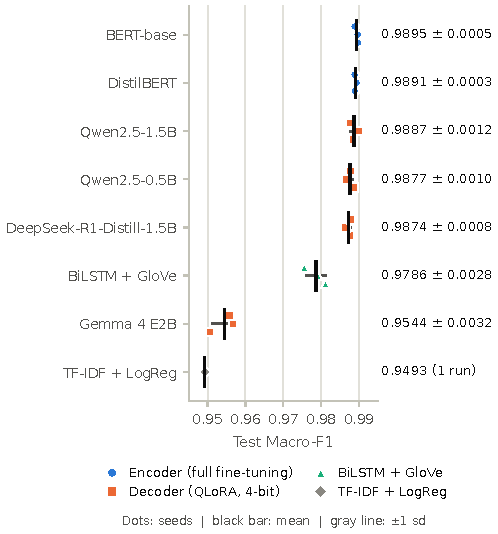
\includegraphics[width=\linewidth]{../results/report/fig_macro_f1.pdf}
\caption{Test Macro-F1 per model: points are seeds, the mark is the mean, and the line is $\pm1$ standard deviation. The Dummy baselines fall outside the plotted range (Table~\ref{tab:main}).}
\label{fig:macrof1}
\end{figure}

\subsection{Controlled Pairs}
Table~\ref{tab:pairs} reports the paired bootstrap. Qwen2.5-1.5B beats Gemma 4 E2B by $0.034$ Macro-F1 on average, and the interval excludes zero in all three seeds with the same sign: the family gap is systematic, although it includes any residual difference between our manual Gemma head and the library head used for Qwen. Between Qwen2.5-1.5B and DeepSeek-R1-Distill-Qwen-1.5B the mean difference is $0.0013$, the interval excludes zero in only one seed, and the sign changes: there is no consistent difference attributable to the training objective, and this pair is also confounded by the base model. Neither scale pair shows a consistent difference. DistilBERT trails BERT-base by $0.0004$ on average and the interval includes zero in all three seeds, so we cannot detect a difference between them. Qwen2.5-0.5B trails Qwen2.5-1.5B by $0.0010$ on average, but the interval excludes zero in only one seed (1337) and the sign changes between seeds; this pair is also confounded by precision (fp16 for the smaller model, bf16 for the larger) and by the machine that trained each.

\begin{table*}[t]
\centering
\caption{Paired bootstrap over the test set (1,000 resamples, 95\% interval, per seed): mean difference in Macro-F1 of A minus B, number of seeds whose interval excludes zero, and whether the sign is the same in all seeds.}
\label{tab:pairs}
\small
% Generado por scripts/make_report.py. No editar a mano.
\begin{tabular}{@{}lrrc@{}}
\toprule
Pair (A vs. B) & Mean $\Delta$ Macro-F1 & Seeds with CI excluding 0 & Same sign \\
\midrule
DistilBERT vs. BERT-base & -0.0004 & 0/3 & no \\
Qwen2.5-0.5B vs. Qwen2.5-1.5B & -0.0010 & 1/3 & no \\
Qwen2.5-1.5B vs. Gemma 4 E2B & +0.0343 & 3/3 & yes \\
Qwen2.5-1.5B vs. DeepSeek-R1-Distill-1.5B & +0.0013 & 1/3 & no \\
\bottomrule
\end{tabular}

\end{table*}

\subsection{Per-Class Results and Error Analysis}
Table~\ref{tab:perclass} shows that for every neural model the three lowest F1 scores are surprise, fear, and anger, while love, despite being a minority class (6.6\%), is among the easiest; Gemma 4 E2B loses most on surprise ($0.9222$ against $0.9798$ for Qwen2.5-1.5B). We analyzed the errors of all eight models; a text counts as an error of a model if it fails it in most of the model's seeds. The five best models make between 258 (BERT-base, 0.69\%) and 335 (DeepSeek-R1-Distill-Qwen-1.5B, 0.90\%) such errors and share many of them: the Jaccard index is 0.62 between the two encoders and 0.54 between Qwen2.5-1.5B and DeepSeek-R1-Distill-Qwen-1.5B. Gemma 4 E2B (1,375 errors, 3.70\%) and TF-IDF (1,620, 4.36\%) are different: 80.1\% and 76.9\% of their errors are made by no other model, against 2\% to 8\% for the five best, which points to a model limitation more than to a property of the data. At the other end, 64 texts (0.17\%) are misclassified by all eight models, and for 22 of them all eight predict the same wrong class. The corpus is made almost entirely of tweets built around ``feel'' (98.5\% of the test texts). The 562 texts without that word (1.5\%) have error rates of 27\% to 35\% for the five best models (46\% for the BiLSTM and 45\% for TF-IDF), against 0.4\% to 0.5\% for the rest; they hold 59\% to 61\% of the errors of the five best models and 86\% of the consensus errors. We read the consensus errors as ambiguous or possibly mislabeled texts, but that is a hypothesis: a manual audit of 30 sampled consensus errors is pending \todo{Audit the 30 texts listed in section 5 of results/errors/cross\_model.md and report the A/B/C counts, or remove the label-noise reading.}

\begin{table*}[t]
\centering
\caption{Per-class F1 on the test set (mean over three seeds).}
\label{tab:perclass}
\small
% Generado por scripts/make_report.py. No editar a mano.
\begin{tabular}{@{}lrrrrrr@{}}
\toprule
Model & Sadness & Joy & Love & Anger & Fear & Surprise \\
\midrule
BERT-base & 0.9942 & 0.9956 & 0.9954 & 0.9871 & 0.9850 & 0.9795 \\
DistilBERT & 0.9941 & 0.9949 & 0.9948 & 0.9863 & 0.9844 & 0.9800 \\
Qwen2.5-1.5B & 0.9946 & 0.9944 & 0.9962 & 0.9850 & 0.9821 & 0.9798 \\
Qwen2.5-0.5B & 0.9932 & 0.9933 & 0.9958 & 0.9828 & 0.9829 & 0.9780 \\
DeepSeek-R1-Distill-1.5B & 0.9931 & 0.9932 & 0.9956 & 0.9835 & 0.9797 & 0.9791 \\
BiLSTM + GloVe & 0.9834 & 0.9852 & 0.9864 & 0.9728 & 0.9751 & 0.9691 \\
Gemma 4 E2B & 0.9753 & 0.9706 & 0.9687 & 0.9466 & 0.9430 & 0.9222 \\
TF-IDF + LogReg & 0.9607 & 0.9641 & 0.9449 & 0.9460 & 0.9454 & 0.9346 \\
Dummy (stratified) & 0.3149 & 0.3509 & 0.0699 & 0.1455 & 0.1085 & 0.0282 \\
Dummy (most frequent) & 0.0000 & 0.5166 & 0.0000 & 0.0000 & 0.0000 & 0.0000 \\
\bottomrule
\end{tabular}

\end{table*}

\subsection{Cost}
Fig.~\ref{fig:cost} plots Macro-F1 against training VRAM and parameters. QLoRA trains between 2.2M and 5.4M parameters (below 0.5\% of the base model), and the decoders peak at 1.2 to 2.7~GB of training VRAM, except Gemma 4 E2B, which needs 9.2~GB and 149 minutes per run for the lowest decoder accuracy. Encoders reach the best Macro-F1 at 1.4 to 2.2~GB and under 17 minutes per run. These numbers come from different GPUs, so we report them per model and do not compare them across machines; we did not measure inference latency.

\begin{figure*}[t]
\centering
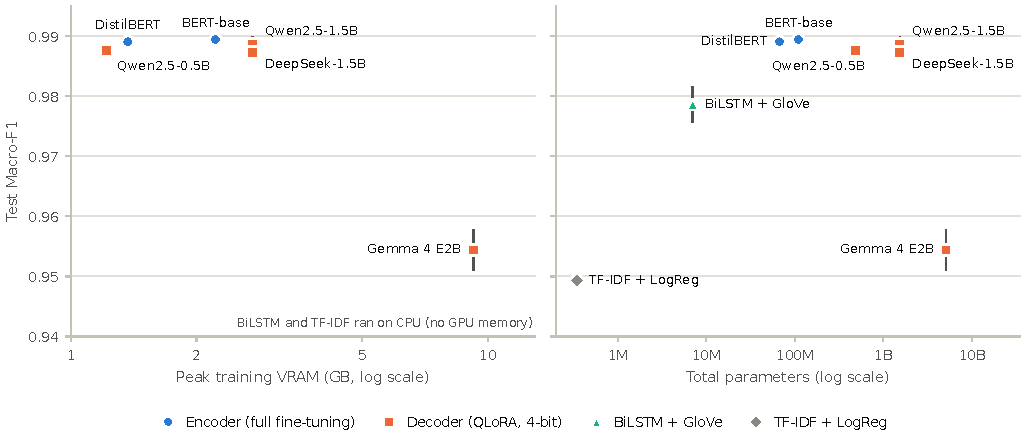
\includegraphics[width=0.8\textwidth]{../results/report/fig_cost_perf.pdf}
\caption{Macro-F1 against training VRAM (left) and total parameters (right). Costs come from different GPUs and are descriptive only.}
\label{fig:cost}
\end{figure*}

\subsection{Explainability of BERT-base}
\label{sec:xai}
We explain BERT-base (seed 42) on 600 test texts sampled by class and on 40 of the 287 errors that this run makes on the test set. The sample is small and the intervals (1.96 standard errors) cover the sampling of texts, not the seed.

\textit{Sanity checks.} Predictions recomputed in fp32 agree with the stored ones in all 640 texts. The completeness error of Integrated Gradients is 1.6\% on average (median 0.2\%, 95th percentile 6.4\%), below our 5\% threshold. Randomizing the whole model removes the agreement with the attributions of the trained model (mean Spearman $\rho=-0.05$, same top word in 4\% of texts). Randomizing only the classification head leaves more agreement in the top word (20\%) although the rank correlation is again near zero ($\rho=-0.12$); this is plausible because the fine-tuned encoder still carries the emotion cues.

\textit{Faithfulness.} Fig.~\ref{fig:faith} compares the methods against random words. Removing the single word with the most attribution changes the predicted class in 75.0\% of the texts and lowers the probability of that class by 0.75 on average, whereas removing one random word changes it in 7.3\% and lowers it by 0.07; with five words the drops are 0.89 and 0.27. Keeping only the top word preserves the decision in 98.5\% of the texts (99.8\% with three words). Attention is much less faithful: removing the top word of the last-layer [CLS] attention lowers the probability by 0.45, and by 0.17 for rollout, which is barely above random. The average drop over $k$ (AOPC \cite{deyoung2020eraser}) is 0.835 for Integrated Gradients, 0.632 for [CLS] attention, 0.363 for rollout, and 0.165 for random words. Removing a word by masking it is not the same as deleting it, since the model never saw such texts in training; this is why random words are the control.

\begin{figure*}[t]
\centering
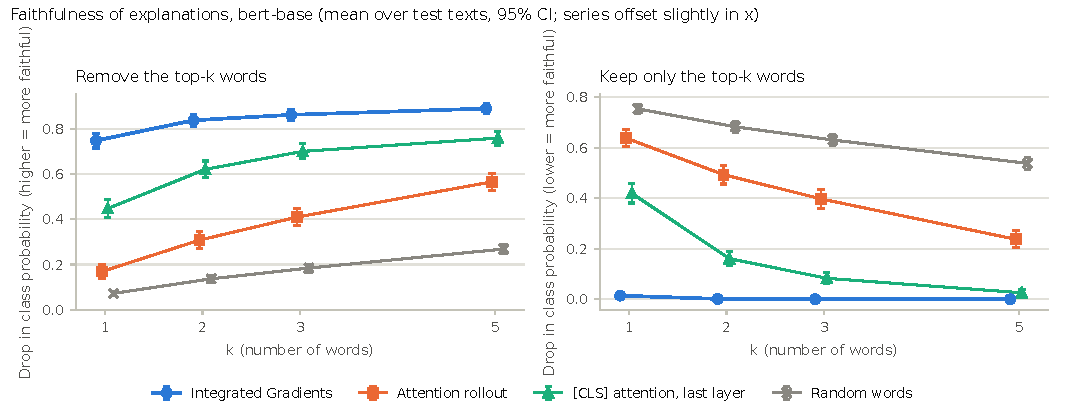
\includegraphics[width=0.85\textwidth]{../results/xai/bert-base/seed_42/fig_xai_faithfulness.pdf}
\caption{Faithfulness of the explanations of BERT-base (seed 42, 600 test texts, 95\% interval). Left: drop in the probability of the predicted class when the $k$ most attributed words are removed. Right: drop when only those $k$ words are kept.}
\label{fig:faith}
\end{figure*}

\textit{Which words the model uses.} The top word of Integrated Gradients is a class-marker word (among the 50 words with the highest log-odds of the predicted class in $S$) in 77.5\% of the texts, against 11.6\% for a random word, 46.2\% for [CLS] attention, and 19.8\% for rollout. It is never a stopword (random words are, in 53.4\%) and it is the word ``feel'' itself in only 2.5\% of the texts; in 95\% of them it comes after the first ``feel'' phrase, so the model mostly reads what follows it. Aggregated over the sample, the most attributed words for love, anger, fear, and surprise are markers (tender, gentle; irritated, insulted; intimidated, afraid; amazed, shocked), while for sadness and joy the aggregate is led by frequent words such as ``feel'' and ``i''. Integrated Gradients and rollout share the top word in 21.5\% of the texts (mean $\rho=0.17$) and Integrated Gradients and [CLS] attention in 51.8\% ($\rho=0.27$). In the last layer, 20.2\% of the [CLS] attention falls on [CLS] and [SEP] (59.7\% for rollout), one more reason to read raw attention with care.

\textit{Errors.} In several of the errors we inspected, the wrong class is driven by one strong emotion word that competes with another. In ``i wasnt feeling that horny just annoyed about work\ldots'' (true class love, predicted anger with probability 0.99), ``annoyed'' pushes toward anger with $+4.48$ and ``horny'' toward love with $+3.82$. In ``i feel so robbed of such a precious life gift'' (true class joy, predicted sadness), ``robbed'' gives $+8.23$ toward sadness and ``precious'' $+7.10$ toward joy. Such texts carry two opposing cues, which fits the hypothesis of ambiguous labels but does not prove it; more examples are in \texttt{examples.html}, next to the other explainability outputs in the repository.

\textit{Reading.} BERT-base decides with very few emotion words placed after ``feel'', and Integrated Gradients flags them faithfully. This is coherent with a TF-IDF model already reaching 0.9493 and with the lexical regularity of the corpus, but it does not show that the model understands emotion. Attributions describe the model, not the cause of the emotion in the text. They depend on a single baseline ([PAD]); other baselines might split the credit differently, and we did not test them.

\section{Limitations}
\label{sec:limits2}
The training subset $S$ is 11\% of the training fold, so the results describe a low-data regime and we did not run a learning curve. The hyperparameter search covers one model per family and its winners for encoders, TF-IDF, and the BiLSTM sit at the grid edge; the decoder search used one epoch, which favors high learning rates. Our learning rate for decoders ($2\times10^{-4}$) lies close to the instability region (rates of $3\times10^{-4}$ and rank 32 collapsed in the search), although none of the twelve final decoder runs collapsed. Machines differ in precision (fp16 on the RTX 2060, bf16 on the RTX 3080), which confounds the Qwen2.5-0.5B vs. 1.5B pair, and costs are not comparable across GPUs. Parameter counts of quantized decoders come from published figures, because the harness under-counts them. The runs of one team member did not record the commit hash. The dataset is almost entirely ``i feel \dots'' tweets, lowercase and unpunctuated, so results may not transfer to other registers, and top models differ by less than the noise of a three-seed estimate. Finally, explainability covers only BERT-base, one seed (42), a sample of 600 texts, and a single [PAD] baseline for Integrated Gradients.


\section{Ethical Considerations}
\label{sec:ethics}

Evaluating emotion classification models on user-generated digital text raises key ethical considerations:
\begin{itemize}
    \item \textbf{Privacy and Anonymization:} The CARER dataset comprises publicly accessible social media posts. All text instances undergo anonymization to scrub personally identifiable information (PII), handles, and explicit user identifiers.
    \item \textbf{Algorithmic Bias and Misclassification:} Emotion classifiers trained on informal digital text can perpetuate demographic or cultural biases. Systemic misclassification of minority affective states could lead to improper downstream actions in sensitive applications such as mental health monitoring.
    \item \textbf{Dual-Use and Psychological Profiling:} Automated affect recognition systems carry risks of unauthorized psychological profiling or manipulative targeted advertising. These models are intended strictly as analytical research baselines.
\end{itemize}

\section{Discussion \& Open Research Directions}
\label{sec:discussion}

\subsection{Architectural Trade-Offs: Performance vs. Memory Footprint}
Section~\ref{sec:results2} is the measured trade-off. Fully fine-tuned encoders reach the highest Macro-F1 at 1.4 to 2.2~GB of training VRAM and under 17 minutes per run. Three of the four QLoRA decoders lie within $0.0021$ Macro-F1 of BERT-base, so parameter scale and the reasoning-distillation objective do not move the result once the adapter and the data are held fixed. The family comparison does: Qwen2.5-1.5B beats Gemma 4 E2B by $0.034$, and Gemma also costs 9.2~GB and 149 minutes for the lowest decoder score. A TF-IDF model already reaches 0.9493, which fits the lexical regularity found by Integrated Gradients. Training costs come from different GPUs and are not comparable across machines. Inference latency was not measured.

\subsection{Handling Imbalance in Parameter-Efficient Regimes}
Class-weighted cross-entropy did not make the smallest classes the hardest. For every neural model the lowest F1 scores are surprise, fear, and anger, while love (6.6\% of the corpus) is among the easiest. The errors of the five best models concentrate on the 1.5\% of test texts that do not contain ``feel''. That pattern is a property of this corpus more than a failure of the minority classes as a group.

\subsection{Future Research Directions}
The open items are those in Section~\ref{sec:limits2}: a learning curve beyond the 32,000-text subset, a hyperparameter search that is not stuck on the edge of the grid, the same precision and GPU for both Qwen sizes, explainability on a decoder, and a second rater for the consensus-error audit. Transfer beyond lowercase ``feel'' tweets, and to other languages or conversational corpora \cite{alam2026beyond, cheng2026personality}, is still untested.

\section{Conclusion}
\label{sec:conclusion}

On a leakage-controlled CARER-derived corpus, eight models trained on the same 32,000 texts and scored on the same 37,153 test texts separate into a tight top group and a clear gap below it. BERT-base is the best model (Macro-F1 $0.9895 \pm 0.0005$), DistilBERT matches it within the seed noise at lower cost, and a paired bootstrap finds a systematic difference only for architectural family (Qwen2.5-1.5B versus Gemma 4 E2B). Scale inside a family and the reasoning-distillation objective do not. The task, as framed by this corpus, is close to saturated for any model that can read the emotion word after ``feel''.

\section*{AI Usage Declaration}
In accordance with institutional guidelines for ethical AI usage in research, the authors declare the use of generative AI tools 
(Claude and Gemini) during the preparation of this manuscript.

AI assistance was used to help draft prose for several subsections after the authors specified the technical content and intended 
argument, to search for and cross-check bibliographic references, to help construct and reconcile comparative tables, and to identify 
and fix LaTeX formatting and compilation issues.

The research question, hypothesis, experimental design, model and dataset selection, and the interpretation of results were determined 
by the human authors. Each author is responsible for manually verifying the bibliographic references and reported results they 
contributed to the manuscript. AI-generated text was reviewed, edited, and approved by the authors before inclusion, and all authors 
remain able to explain and defend every decision, source, and claim in this document.
\bibliographystyle{IEEEtran}
\bibliography{references}

\end{document}
